\documentclass{VUMIFPSkursinis}
\usepackage{algorithmicx}
\usepackage{algorithm}
\usepackage{algpseudocode}
\usepackage{amsfonts}
\usepackage{amsmath}
\usepackage{bm}
\usepackage{caption}
\usepackage{color}
\usepackage{float}
\usepackage{graphicx}
\usepackage{listings}
\usepackage{subfig}
\usepackage{wrapfig}


% Titulinio aprašas
\university{Vilniaus universitetas}
\faculty{Matematikos ir informatikos fakultetas}
\department{Programų sistemų katedra}
\papertype{Kursinis darbas}
\title{Mobiliųjų programų testavimas remiantis TMMi modeliu.}
\titleineng{TMMi model based mobile application testing.}
\status{3 kurso 4 grupės studentas}
\author{Ričardas Mikelionis}
\supervisor{Lekt. dr. Vytautas Valaitis}
\date{Vilnius – \the\year}

% Nustatymai
\setmainfont{Palemonas}   % Pakeisti teksto šriftą į Palemonas (turi būti įdiegtas sistemoje)
\bibliography{bibliografija}

\begin{document}
\maketitle

\cleardoublepage
\pagenumbering{gobble}
\tableofcontents
\cleardoublepage
\pagenumbering{arabic}

\sectionnonum{Įvadas}
Nuo 2007, kai buvo pristatytas pirmasis iPhone jau praėjo kiek daugiau nei dešimt metų. Šio mobiliojo įrenginio, išmaniojo telefono (angl. Smartphone), pristatymas  iš esmės pakeitė mobiliųjų kompiuterių rinką. Iki tol asmeniniai skaitmeniai asistentai (angl. PDA personal digital asistant) buvo nei prieinami, nei labai naudingi įprastam vartotojui, todėl juos turėjo keletas verslo pasaulio žmonių, o paprastas vartotojas su savimi nešiojosi krūvą skirtingą funkcionalumą atliekančių prietaisų: MP3 grotuvų, Fotoaparatų, nešiojamųjų kompiuterių, telefonų. iPhone žadėjo delne telpantį kompiuterį kiekvienam už prieinamą kainą, ir savo pažadą įvykdė. Vienas po kito ėmė rastis  mobiliosios operacinės sistemos, turėjusios tiesiogiai konkuruoti su iPhone naudojama iOS,  kaip PalmOS, Symbian, Windows 7 mobile, vėliau tapusi 8 ir 8.1 bei Android. Mobiliųjų kompiuterių bei telefonų rinką užplūdo krūvos prieinamų įrenginių, kurie su kiekviena nauja laida savo skaičiavimo sugebėjimais artėja arčiau ir arčiau to ką gali atlikti staliniai kompiuteriai, ir iš pažiūros 2017 metų išmanusis įrenginys savo specifikacijomis „ant popieriaus“ jau seniai pranoko 2007 metų kompiuterį.

Nors šiandien iš gausaus operacinių sistemų pasirinkimo rinkoje iš esmės išlikę tik dvi: iOS ir Android, tačiau  išmaniųjų prietaisų populiarumas toli gražu neblėsta. 2016 metais pasaulyje jau buvo apie 2.1 mlrd. išmaniųjų telefonų naudotojų, o iki 2020 planuojama, jog šis skaičius sieks 2.87 mlrd.\cite {statista.com}. Esant didžulei įrenginių paklausai proporcingai kyla poreikis ir programinei įrangai pritaikytai šiems įrenginiams - mobiliosioms programoms.

Šio darbu siekiama pateikti esminius skirtumus tarp įprastų darbastalio (angl. desktop) bei internetinių (angl. Web) programų ir mobiliųjų programų skirtų išmaniesiems įrenginiams kokybės užtikrinimo. Šio darbo tikslas - išanalizavus dabartinės rinkos mobiliųjų programų kūrimo procesų tendencijas, išskirti problemines mobiliųjų programų kokybės užtikrinimo sritis bei pateikti keletą probleminių sričių kokybės užtikrinimo sprendimų remiantis testų brandos modeliu.

Siekiant sėkmingai įgyvendinti užsibrėžtą dabo tikslą darbo metu bus:
\begin{itemize}
   \item Atliekama mobiliųjų įrenginių sampratos analizė, siekiant išsiaiškinti esminius skirtumus, kurie gali daryti įtaką mobiliųjų programų veikimui;
   \item Remiantis mobiliųjų įrenginių sampratos analize išrenkamos pagrindinės probleminės sritys mobiliųjų programų testavime;
   \item Atliekama integruotojo testų brandos modelio - TMMi detali analizė;
   \item Remiantis mobiliųjų programų testavimo probleminėmis sritimis bei TMMi analizės rezultatais pateikiamas TMMi paremtas modelis skirtas padengti visas problemines sritis;
   \item Atliekama agiliųjų metodikų naudojimo mobiliųjų programų kūrime apžvalga;
   \item Remiantis agiliųjų metodikų iteratyvumu pateikiamas TMMi modelis pritaikytas komandoms dirbančioms pagal agiliasias metodikas.
\end{itemize}



\section{Mobiliųjų programų kokybės užtikrinimas.}

2013 metais atliktas tyrimas \cite {compuware.com} rodo, jog 79\% išmaniųjų telefonų naudotojų išbando atsisiųstą programėlę tik kartą prieš ištrindami. Didelė to priežastis yra žemesnė mobiliųjų programų kokybė palyginus su tuo ką vartotojai yra įpratę matyti savo naršyklėse, ar darbastalio programose. Išmaniųjų telefonų naudotojai yra pratę prie nemokamos ar žymiai mažiau kainuojančios programinės įrangos, kuri gauna nuolatinius atnaujinimus. (Pvz.: Adobe photoshop express iOS 0eur., Adobe Photoshop Windows 10 290eur./m. \cite{adobe.com}). Kyla kainų dilema: norint palaikyti žemas kainas rinkoje reikia mažinti kainas ir kūrimo procese. Tai dažnai daroma taupant laiką, kur ir nukenčia kokybės užtikrinimo procesai.

Į mobiliųjų programų kūrimą vis dar žiūrima taip pat, kaip į interneto programų (angl. WEB application) ar darbastalio programų kūrimą, neįžvelgiant esminių skirtumų tarp šių dviejų programinės įrangos kūrimo procesų. Didžiulė įrenginių variacijų gausa, ir iš esmės išsiskiriantys naudojimosi mobiliąja programine įranga įpročiai turėtų versti kūrėjus į mobiliųjų programų kūrimą žvelgti kitaip.

\subsection{Mobiliųjų programų kūrimo proceso probleminės sritys.}
M. Satyanarayanan dar 1996-aisiais savo straipsnyje apie mobiliuosius kompiuterius puikiai aibrėžė esmines sritis, kurios išskiria mobiliuosius įrenginius nuo stacionariųjų. Išskirtos keturios sritys \cite{Satyanarayanan:1996:FCM:248052.248053}:
\begin{itemize}
   \item Riboti skaičiavimo ištekliai (angl. limited computing resources)
   \item Apsauga ir pažeidžiamumas
   \item Galia (angl. performance) ir patikimumas
   \item Riboti energijos ištekliai.
\end{itemize}

Iš esmės mobiliosios programos yra tokia programinė įranga, kuri veikia nešiojamame (mobiliame) įrenginyje. Tačiau į mobiliąją kompiuteriją žvelgiant per išmaniųjų telefonų prizmę mobiliųjų programų apibrėžimą galime sukonkretinti. Mobilioji programa (angl. mobile app) - programa suprojektuota veikti išmaniąjame telefone, planšetiniame kompiuteryje ar kitame mobiliame įrenginyje ir/arba, kaip įvestį, priimanti situacija paremtą (angl. context based) informaciją pvz. GPS signalas. \cite{6496451} Situacijos supratimas, naudojimasis situacine informacija ir gabėjimas keisti programos elgseną pagal gautus duomenis yra dar vienas esminis mobiliųjų programų, ypač skirtų išmaniesiems telefonams, skiriamasis bruožas.

Remiantis šiais keturiais techniniais išskirtinumo bruožais, ir esminiu veikimo skirtumu galima pradėti išskirti problemines kokybės užtikrinimo sritis mobiliųjų programų kūrime. Laikant progamas išmaniesiems telefonams tyrimo baziniu objektu išskiriamos šios sritys:
\begin{itemize}
  \item  Ryšio sujungiamumo
  \item Ribotų išteklių
  \item Draugiškumo vartotojui
  \item Situacinio prisitaikymo
  \item Įrenginių gausos
  \item Naujų operacinių sistemų versijų
  \item Liečiamųjų ekranų
\end{itemize}

\subsubsection{Ryšio sujungiamumo probleminė sritis}
Sugebėjimas prisijungti prie mobiliojo ryšio stočių bei bevielio interneto taškų dažnai mobiliajai programai yra kritinis reikalavimas be kurio ši nesugebės funkcionuoti. Problema kyla dėl ryšio nepastovumo keliaujant. Keliaujant didelius atstumus vyksta persijungimai tarp mobilaus ryšio stotelių, vartotojas gali pakliūti į neryšio zoną, ar vietą kurioje veikia viso labo GPRS ar EDGE ryšys. Taip pat ir su bevielio interneto stotelėsmis, kurių dažna veikia vos 100m. spinduliu nesant jokiems trukdžiams. 

Testuojant šioje srityje derėtų atsižvelgti į jau egzistuojančius ryšio defektus esančius specifiniame testavimui naudojamame įrenginyje, ar operacinėje sistemoje. \cite{android_bugs} Testuojant programas kurios smarkiai remiasi į įrenginio sugebėjimą prisijungti prie interneto ar mobiliojo ryšio tinklų atsiranda poreikis atlikti funkcinius testus įvairuose ryšio sujungiamumo scenarijuose. Pagrindinis siekis yra užtikrinti teisingą programos veikimą, net dingus ryšiui ar šiam staiga smarkiai sulėtėjus.

\subsubsection{Ribotų išteklių probleminė sritis}
Kol mobilieji įrenginiai tampa vis galinesni ir galingesni, jie vis dar negali pasivyti satcionariųjų bei nešiojamųjų kompiuterių. Pavyzdžiui vienas iš galingesnių šiuo metu rinkoje esančių telefonų, Samsung Galaxy s8+ turi 6GB atminties bei 8 branduolių, palaikančių 8 gijas, sistemą mikroschemoje (angl. system on a chip) į kurią integruoti vaizdo procesorius bei pagrindinis procesoriai. \cite{samsung_s8} Šiuo metu didžioji dauguma vartotojams prieinamų motininių plokščių kompiuteriams palaiko iki 64GB atminties, o intel neseniai atskleidė savo naujosios kartos i9 procesorių liniją, kur aukščiausios klasės procesorius sudarytas iš 18 branduolių bei 36 gijų. \cite{intel_i9}

Testuojant šioje srityje būtina atsižvelgti į išteklių įrenginyje naudojimą paleidžiant bei naudojant programą. Tai daroma siekiant išvengti staigių našumo sumažėjimų, neteisingo, nenumatyto programos ar įrenginio veikimo staiga imant naudoti 100\% prieinamų išteklių. Pagrindinis testavimo siekis užtikrinti teisingą programos bei įrenginio veikimą esant skaičiavimo išteklių trūkumui.

\subsubsection{Draugiškumo vartotojui probleminė sritis}
Kūrėjai kuriantys programas mobiliosioms operacinėms sistemos (Android, iOS) privalo sekti operacinių sistemų kūrėjo nusatytas varotojų sąsajos gaires. Dėl įrenginių gausos, skirtingų dydžių bei raiškos ekranų atsiranda grafinių neatitikimų tikimybė. 

Testuojant šioje srityje būtina testavimą atlikti ant daug skirtingų įrenginių, veikiančių su skirtingomis operacinės sistemos versijomis bei skirtingų raiškų bei dydžių ekranais.

\subsubsection{Situacinio prisitaikymo probleminė sritis}
Didelė dalis mobiliųjų programų remiasi duomenimis gautais priklausomai nuo situacijos, iš įvairių sensorių išmaniajame įrenginyje. Dažnai išmanieji įrenginiai turi įvairių sensorių, kaip, mikrofonai, šviesos jutikliai, akselerometrai bei giroskopai, vaizdo kameros. Tokie įrenginiai turi ir keletą būdų komunikuoti, susijunti su kitais prietaisais, internetu: bluetooth, wifi, 4G/LTE, NFC. Visi šie sensoriai gali suteikti prigramai krūvą informacijos realiu laiku, atsižvelgiant į tai ką vartotojas veikia su įrenginiu, ar kur jis tuo metu yra.

Testuojant šioje srityje patikrinti visų įrenginių ir įvesčių kombinacijų praktiškai neįmanoma. Todėl testus reikia skirstyti į kontekstinius (angl. context-specific), bei nusistatyti užtektinus testų padengtumo kriterijus. Kuriant kontekstu paremtus testus, bei renkantis įrenginius su kuriais bus vykdomi testavimo atvejai verta atsižvelgti į konkrečiam įrenginiui būdingus ar operacinės sistemos versijai būdingus defektus. \cite{android_bugs}

\subsubsection{Įrenginių gausos probleminė sritis}
Rinkoje, vartotojams prieinami šimtai skirtingų mobiliųjų įrenginių iš skirtingų gamintojų, veikiančių su skirtingomis operacinėmis sistemomis, surinktų iš skirtingų komponentų. 2013 metais atlikto tyrimo metu buvo suskaičiuota, jog rinkoje yra apie 1800 unikalių vien Android operacine sistema paremtų įrenginių modelių. \cite{Muccini:2012:STM:2663608.2663615}

Testuojant šioje srityje reikia stengtis maksimizuoti testų padengtumą minimizuojant naudojamų įrenginių kiekį. Tą galima daryti grupuojant įrenginius, ir testuojant ne konkrečiuose įrenginiuose (mažiau įrenginių) tačiau grupėse. Pavyzdžiui:

\begin{itemize}
   \item Pirmoji grupė, žemiausio prioriteto testai, silpni, palyginus su dabartiniais pagrindinių gamintojų flagmanais, turintys silpnesnius procesorius, mažiau atminties, žemesnės raiškos ekranus. Paremti senesne operacinės sistemos versija, veikiantys su senesne naršykle. Dar vis populiarūs, tačiau gamintojo jau nebepalaikomi įrenginiai.

   \item Antroji grupė, vidutinio prioriteto testai, vidutinio galingumo įrenginiai, dažniausiai kelių iteracijų, palyginius su dabartiniais pagrindinių išmaniųjų įrenginių gamintojų flagmanais, senumo pvz: iPhone 5s palyginus su iPhone 7. Jau gan seni, 3-2 metai, tačiau dar vis gamintojo palaikomi įrenginiai.

   \item Trečioji grupė, patys naujausi <1 metų senumo įrenginiai. Paremti naujausia operacinės sistemos versija, naujausios kartos komponentais, turintys daugiau atminties, aukštesnės raiškos ekranus, nei praeitos iteracijos modeliai.\cite{6496451}
\end{itemize}

Testuojant pasirinkta įrenginių kombinacija įgalina keletą pasirinkimų, kaip tokį testavimą galima vykdyti: naudoti rankinį testavimą ar automatinį testavimą, testavimui pasitelkti komandas įmonėje ar žmones pasamdytus iš kitų įmonių, testuoti pagal planą ar naudoti tiriamąjį testavimą (angl. exploratory testing) bei naudoti emuliatorius, virtualias mašinas ar testuoti ant realių, fizinių įrenginių.

\subsubsection{Naujų operacinių sistemų probleminė sritis}
Mobiliosios operacinės sistemos, palyginus su operacinėmis sistemomis stacionariesiems kompiuteriams, yra išleidžiamos labai dažnai. Pastaruoju metu tiek iOS tiek Android nauja „numeruotoji“ versija yra išleidžiama kas met. Taip dažnai išleidžiant naują operacinės sistemos iteraciją gali kilti daugybė nesuderinamumo defektų, turint omenyje tai, kad ne visos versijos yra palaikomos, t.y. naujesnės programų versijos gali veikti tik su keliomis paskutinėmis operacinės sistemos iteracijomis.

Testuojant programas reikėtų atsižvelgti į egzistuojančius konkrečios operacinės sistemos versijos defektus, bei testuoti naudojant keletą skirtingų tos pat operacinės sistemos iteracijų. Taip siekiant įsitiktinti, ar defektai atsiradę mobiliojoje programoje buvo sukelti operacinės sistemos defekto, ar blogo kodo.

\subsubsection{Liečiamųjų ekranų probleminė sritis}
Liečiamieji ekranai yra pagrindinis, ir dažniausiai vienintelis įvesties pateikimo būdas mobiliuosiuose įrenginiuose. Dažna problema, ypač senesniuose įrenginiuose, yra lėtas prisilietimo prie ekrano atsakas, ar ekrano įvesties atsako laiko padidėjimas imant naudotis sudėtingesnėmis programomis.

Testuojant reikėtų naudoti daug skirtingų įrenginių, kurie iš esmės skiriasi savo specifikacijomis, ypač ekranų dydžiu, raiška. Pagrindinis testavimo objektas yra resursų pasiskirstymas. Tikrinama ar testuojama programinė įranga mobilajame įrenginyje „neryja“ resursų. Reikėtų stengtis įvykdyti didelės apkrovos scenarijų, kai programinė įranga veikia pilnu pajėgumu atlikdama didžiausių skaičiavimų reikalaujančias užduotis, ir tikrinti mobiliojo įrenginio atsako laiką.

\subsection{Integracinis testų brandos modelis - TMMi}
Testų brandos modelis buvo sukurtas, tam, kad įvairios organizacijos galėtų įvertinti bei įvertinę pagerinti savo testavimo procesus. Tai taip pat teikia naudą, kaip modelis, tiesiogine to žodžio prasme, kuris nurodo, kaip testavimo procesas turėtų  palaipsniui gerėti savo efektyvumu bei kokybe. \cite{Burnstein:2010:PST:1965566} Žinoma, jog TMMi nėra vienintelis procesų vertinimo bei gerinimo modelis ar standartas, per paskutiniuosius du dešimtmečius buvo sukurti ne vienas toks standartas. Vienas iš jų yra CMM - Gebėjimo Brandos Modelis (angl. Capability Maturity Model) bei jo įpėdinis Integruotas Gebėjimo Brandos Modelis (angl. Capablitiy Maturity Model Integration - CMMi). Tačiau palyginus su TMM bei TMMi daugelis šių modelių neskiria pakankamai dėmesio testavimo procesų gerinimui. 

TMMi modelis sudarytas iš penkių brandos lygių, kurie kiekvienas rodo testavimo proceso brandos būseną. Šie modelio nustatyti lygiai padeda struktūrizuotai siekti aukštesnio proceso našumo, taigi jų reikia siekti iš eilės t.y. negalima iš antro brandos lygio iš karto pasiekti ketvirtojo ar penktojo. Taip pat struktūrizuotas išskirstymas lygiais užtikrina, jog pasiekus aukštesnyjį lygį žemesniajame lygyje pradėtos naudoti praktikos bus naudojamos ir toliau.

Kiekvienam testų brandos lygiui pasiekti užsibrėžiamos veiklos, užduotys bei pareigos (angl. Activities, Tasks, Responsibilities - ATR). Šie trys kriterijai nurodo esmines sritis kurios turi būti įtrauktos į testavimo procesą, tam, kad būtų pasiektas norimas brandos lygis. Šie brandos tiksliai turi tapti siekiamybe visiems kūrimo procese dalyvaujantiems žmonėms, ne tik kokybės užtikrinimo srities specialistams. Taip užtikrinimas visapusiškas testavimo proceso palaikymas bei įvertinimas siekiant pagerėjimo.

Testų brandos lygis nustatomas naudojantis TMMi įvertinimo modeliu (angl. TMMi assessment model) sudatyto iš trijų komponentų.
\begin{itemize}
   \item Klausimyno, susijusio su brandos tikslų siekimu. Skirt nustatyti dabartinę testavimo proceso būsesną.
   \item Gairių rinkino skirto įvertinimo komandai.
   \item Įvertinimo procedūra išdėstyta pažingsniui, skirta vesti įvertinimo komandą per testų procesų įvertinimą bei gerinimą.
\end{itemize}

\subsubsection{Testų Brandos Modelio testų brandos lygiai}
Testų brandos modelį apibrėžia penki brandos lygiai\cite{Burnstein:2010:PST:1965566}:
\begin{enumerate}
   \item Pradinis (angl. Initial)
   \item Fazių aiprėžimo (angl. Phase definition)
   \item Integracijos (angl. Integration)
   \item Valdymo bei vertinimo (angl. Management and Measurement)
   \item Optimizacijos arba Defektų prevencijos bei kokybės valdymo (angl. Optimisation/Defect Prevention and Quality Control)
\end{enumerate}
Kiekvienas iš šių lygių turi ir vidinę struktūrą Priedas nr. 1. Pirmasis brandos lygis savo struktūros neturi, nes tiesiog nurodo bazinio proceso egzistavimą, o jo pasiekimui užtenka chaotiško proceso. Kiekvieno brandos lygio brandos tikslai atspindi testavimo proceso pagerinimo tikslus, kuriuos reikia įvykdyti norint pasiekti norimą brandos lygį. Taip pat norint pasiekti aukštesnį lygį būtina įgyvendinti ir visus tikslus reikalingus pasiekti žemesnius lygius tam, kad nevyktų proceso brandos regresija ir tikrai būtų pasiektas testavimo proceso pagerinimas.\cite{Tmmi}

\subsubsubsection{Pirmasis brandos lygis}
Šiame brandos lygyje operuoja visos programinės įrangos kūrėjų komandos, kurios turi bet kokį testavimo procesą. Pasiekti šį lygį užtenka chaotiško, neefektyvaus, tačiau vykdomo testavimo proceso. Šiame lygyje testai dažniausiai būna pritaikyti konkrečiai situacijai, nėra kartotini. Testavimo procesas iš esmės neturi kokybės standarto.

\subsubsubsection{Antrasis brandos lygis}
Šiame brandos lygyje iš chaotiško proceso imamas apibrėžti konkretus testavimo metodas, bei testavimo procesas imamas valdyti. Imami apibrėžti testavimo scenarijai, kuriami testavimo planai, dažniausiai iš reikalavimų yra keliami testavimo atvejai. TMM bei TMMi paremti krioklio (angl. waterfall) metodologija, todėl testavimas dažniausiai atliekamas kūrimo proceso gale, lyginant turimą produktą, su kūrimo pradžioje apibrėžtais reikalavimais. Pasiekę šį lygį dar, savaime aišku, neturime visiškai efektyvaus testavimo proceso, tačiau turime konkrečiai apibrėžtą testavimo proceso kryptį, kurią bus galima toliau plėtoti siekiant aukštesnio testavimo proceso brandos lygmens.

\subsubsubsection{Trečiasis brandos lygis}
Šiame brandos lygyje apibrėžiamas standartizuotas procesas bei procedūros, kurios bus naudojamos, visoje organizacijoje, komandoje, kurios testavimo procesą stengiamasi pagerinti. Pasiekus antrąjį brandos lygį testavimo procesas yra struktūrizuotas čia jis imamas integruoti į programinės įrangos kūrimo gyvavimo ciklą (angl. Developement life cycle). Pasiekus trečiąjį testavimo proceso bandos lygį, antrąjame apibrėžtas procesas bus integruotas ir pradėtas naudoti visuose naujuose projektuose nuo pat projekto pradžios. Šiame lygyje dar dažnai planuojamas bei vykdomas nefunkcinis testavimas kiekviename projekte įtrauktame į testavimo procesą.

\subsubsubsection{Ketvirtasis brandos lygis}
Pasiekus šį brandos lygmenį, visų kūrimo veiklų bei rezultatų detalus vertinimas. Procesų vertinimas turėtų būti pradėtas vykdyti nuo pačios anksčiausios kiekvieno projekto stadijos. Taip siekiama kiekvieną projektą įgyvendinti su kuo įmanoma mažiau defektų. Šiame lygyje vykdomos išsamios projekto apžvalgos, bei ankstyvose projektų stadijose vykdomas statinis testavimas derinamas su dinaminėmis testavimo technikomis apibrėžtomis antrąjame testų proceso brandos lygyje. Pasiekus šį brandos lygį testavimo procesas vykdomas visuose programinės įrangos kūrimo gyvavimo ciklo etapuose, taip pat įtraukiant produktų dokumentacijos peržiūrą Priedas nr. 2. Pakankamos kokybės kriterijai apibrėžiami visiems produktams toje organizacijoje.

\subsubsubsection{Penktasis brandos lygis}
Šiame brandos lygyje visos testavimo veiklos bei rezultatai yra vertinami siekiant juos optimizuoti. Tai daroma norint nuolatos tobulinti testavimo procesą siekiant visiškos defektų prevencijos, o ne defektų taisymo.

\subsubsection{Testų Brandos Modelis TMM bei Gebėjimo Brandos Modelis CMM}
Gebėjimo brandos modelis iš pradžių buvo sudarytas, kaip įrankis objektyviai bei tiksliai įvertinti valstybinių projektų vykdytojų darbo procesų kokybę įgyvendinant užsakytą programinės įrangos projektą. Šis modelis smarkiai paremtas procesų brandos modeliu pirmą kartą aprašytu W.Humphrey knygoje „Managing the software Process“. \cite{Paulk:1993:CMM:624600.625307}

TMM modelio struktūra yra paremta tuo kas buvo sukurta CMM modeliui, todėl abiejuose modeliuose randamos tokios pat esminės sudedamosios dalys, kaip pavyzdžiui brandos lygiai su panašiais, o kai kur ir identiškais tikslais tam lygiui pasiekti. Pažvelgus į CMM modelį kyla klausimas ar juo vertėtų naudotis šiandien, gerinant testavimo procesų kokybę nuosavame projekte? CMM ir kiti panašūs modeliai (ISO 9001, BOOT-STRAP, SPICE) tinkamai neatsižvelgia į testavimo keliamas problemas, todėl nėra tinkami konkrečių testavimo procesų gerinimui, tačiau verta pažvelgti giliau į tai, kaip CMM modelis buvo pakeistas kuriant TMM modelį.

Pagrindiniai CMM bei TMM skirtumai:
\begin{itemize}
   \item Gebėjimo brandos modelyje testavimo proceso branda nėra apibrėžta.
   \item Pagrindinės testavimo probleminės sritys nėra apibrėžtos esminiuose procesuose.
   \item Nedaug dėmesio skiriama aukštos kokybės testavimui, kaip procesų bei produktų gerinimo strategijai.
   \item Nepilnai apibrėžiami, ne daug minimos su kokybe susijusios problemos kaip testuojamumas, testų pakankamumo kriterijai, testavimo planavimas bei programinės įrangos sertifikavimas.
   \item Pažangesni testavimo procesai, kaip vartojimo statistikos surinkimas, statistinis testavimas bei kiekybinė testavimo proceso kontrolė yra nepakankamai aprašyti.
\end{itemize}
Šiandien testavimas programinės įrangos kūrimo procesuose atlieka labai svarbų vaidmenį, todėl jam teikiamas toks pat, jeigu ne didesnis dėmesys, kaip programinės įrangos kūrimui. Turint tai omenyje, CMM bei jo įpėdinis CMMi tampa nepriimtini dėl dėmesio testavimo procesų gerinimui stokos.

\subsection{Probleminių sričių pasiskirstymas TMMi modelyje.}
TMMi savo lygmenimis išskirsto ir funkcinį bei nefunkcinį testavimą, pvz. Antrąjame lygyje užtenka sutvarkyti funkcinio testavimo procesus, o trečiojo lygio nebus galima pasiekti neįgyvendinus nefunkcinio testavimo proceso tvarkos. Auščiau išskirtas mobiliųjų programų testavimo problemines sritis taip pat paprastai galima išskirstyti į funkcinio testavimo bei nefunkcinio testavimo rūšis:
\begin{itemize}
   \item Funkciniai testai: Draugiškumo vartotojui probleminė sritis, Situacinio prisitaikymo probleminė sritis bei Įrenginių gausos probleminė sritis.
   \item Nefunkciniai testai: Ribotų išteklių probleminė sritis, Ryšio sujungiamumo probleminė sritis.
\end{itemize}
Kadangi probleminių sričių testavimas lengvai išskirstomas į funkcinį bei nefunkcinį, jam galima nesunkiai pritaikyti testų brandos modelį. Taip ne tik pasiekiant pilną probleminių sričių padengtumą testais, tačiau ir bendro testavimo proceso pagerinimą.

\begin{figure}[H]
    \centering
    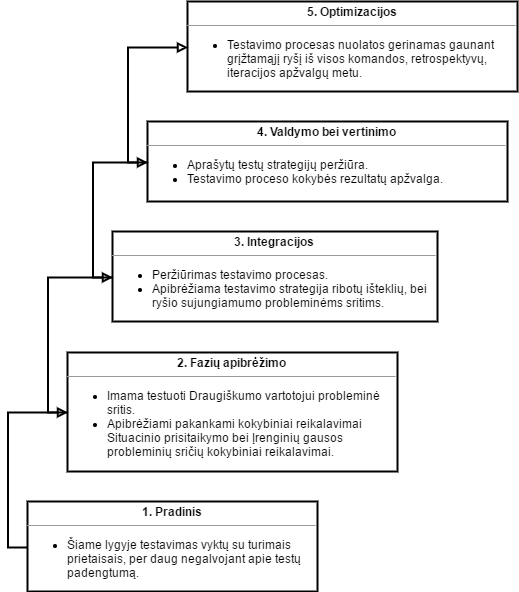
\includegraphics[scale=0.85]{img/Tmmimobile}
    \caption{Mobiliojo testavimo probleminės sritys sudėtos į TMMi brandos modelį.}
    \label{img:tmmimobile}
\end{figure}

\section{Agile metodologijos mobiliųjų programų kūrime.}
Agilieji kūrimo metodai (angl. agile) tai lanksčios programinės įrangos kūrimo metodikos. Tokiose metodikose viskas kūrimo procesas yra suskaldomas į eilę ciklų, dar vadinamų iteracijomis. Dažnai, kuriant mobiliasias programas remiantis agiliaisiais metodais, visos užduotys padalijamos į keletą mažesnių, skirtų įvykdyti didesniąjai, kurių kiekviena tampa kone savo atskiru mikroprojektu iš kurio pro iteracijos komanda gauna veikiančio produkto dalį.

Iteracinis išskirstymas leidžia projektą tvarkingai išskirstyti logiškai, viena po kitos einančiomis dalimis, taip pat išskirstant komandos resursus atitinkamai dirbti mažesnėse komandose, taip sumažinant kūrimo rizikas, tokias, kaip defektai.

\subsection{TMMi ir Agile}
Testų brandos modelis bei agiliosios kūrimo metodologijos, dvi praktikos, kurios skiekia to paties, tačiau iš pirmo žvilgsnio nėra suderinamos. TMMi, kaip ir daugelis kitų brandos modelių, yra paremtas V modeliu Priedas nr. 2, tai tokia programinės įrangos kūrimo metodologija, kai  visi planavimo, kūrimo bei testavimo procesai yra vykdomi atskirai vienas nuo kito, paeiliui, o kūrimo metu tik planuojant testavimą. Kol tuo tarpu agiliųjų metodologijų manifeste teigiama, jog žmonės ir bendravimas vertinamas labiau, nei procesai ar įrankiai, veikianti programinė įranga vertinama labiau, nei išsami dokumentacija, bendradarbiavimas su klientu vertinamas labiau, nei derybos dėl kontraktų ir reagavimas į pokyčius vertinamas labiau, nei plano įvykdyamas \cite{agile}. Iš pirmo žvilgsio abi metodologijos atrodo visiškomis priešingybėmis. Ar galime daryti išvadą, jog agiliųjų metodologijų testavimo procesas pasmerktas ir nepagerinamas?

Kuriant programinę įrangą agiliosiomis metodologijomis, nėra rašoma palti dokumentacija, tačiau kiekvienos iteracijos pradžioje imama dalis reikalavimų, užduočių, ir detaliai išnagrinėjiama įvertinama valandų kiekiu, ar pagal sudėtingumą, o kiekvienos iteracijos pabaigoje vyksta apžvalga, aptarimas skirtas pagerinti procesus kitai iteracijai bei apptarti, kas buvo nuveikta šią iteraciją.

Naudojantis agiliosiomis metodologijomis nėra kuriamas detalus testavimo planas visam projektui, komanda pati neapibrėžia kokybės reikalavimų kiekvienai užduočiai. Testai kuriami universalūs, pritaikomi kiekvienai iteracijai, papildomi naujo funkcionalumo testais atitinkamai nuo to, kas yra atlikta, ar planuojama atlikti. Kokybiniai reikalavimai kinta, tačiau yra lengvai nustatomi glaudžiai bendradarbiaujant su projekto užsakovu, ką agiliosios metodologijos ir skatina.

Žvelgiant į kiekvieną agiliąją iteraciją, kaip atskirą projektą, jai galima pritaikyti V-modelį, o tuo labiau TMMi testų brandos modelį. Remiantis išskirtais TMMi lygiais, aglijiuoju manifestu bei tokio kūrimo procesu agilųjį testavimo procesą TMMi modelyje butų galima išdėstyti taip:

\begin{figure}[H]
    \centering
    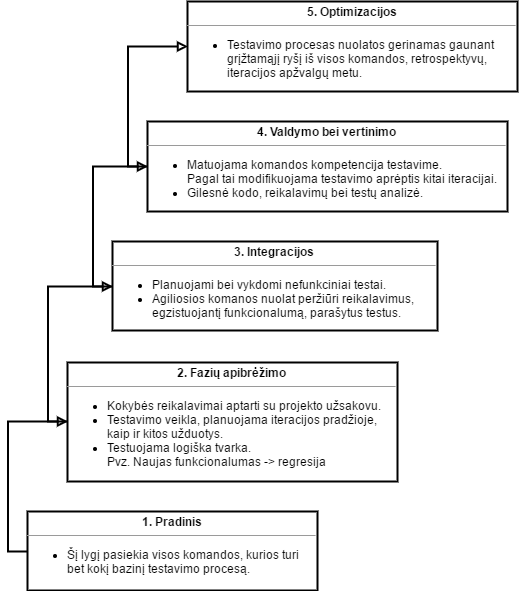
\includegraphics[scale=0.85]{img/Tmmagile}
    \caption{Agile metodologijos įpatumai sudėti į TMMi brandos modelį.}
    \label{img:tmmiagile}
\end{figure}

\sectionnonum{Rezultatai ir išvados}
Šiame darbe buvo išnagrinėtas programinės įrangos kūrimas remiantis mobiliojo įrenginio apibrėžimu, taip išskiriant esminius skirtumus tarp programinės įrangos kūrimo mobiliesiems įrenginiams bei programų kūrimo stacionariems kompiuteriams, interneto programų kūrimo.

Atliekant tyrimą pastebėta, jog informaciją apie mobiliųjų programų kūrimą visada pateikiama per agiliųjų metodologijų prizmę, tačiau testų procesų gerinimo metodai, testų brandos modeliai, yra paremti V-modelio programinės įrangos kūrimo metodologijomis. Buvo pasirinkta strategija išskirti problemines mobiliųjų programų testavimo sritis, tuomet jas pritaikyti TMMi modeliui priskiriant atitikamam brandos lygmeniui. Ta pati strategija buvo taikoma atskirai nagrinėjant agiliasias metodologijas, siekiant rasti sprendimą, kai V-modeliu paremtas testų brandos modelis galėtų būti pritaikomas su agiliosiomis praktikomis.

 Šiame darbe didžiausias demesys buvo skirtas mobiliųjų programų, skirtų išmaniesiems įrenginiams tokiems, kaip išmanieji telefonai, planšetiniai kompiuteriai, kūrimo procesui. Priežasčių, kodėl tokių programų kūrimo procesas daugelyje komandų būna neefektyvus, tyrimui. Išsiaiškinus šias priežastis, buvo siekta ieškoti sprendimų, pritaikant jau atliktus konkrečius tyrimus nagrinėjančius mobiliuosius įrenginius, mobiliųjų programų kūrimą bei testų brandos modelio taikymą, taip apjungiant naudingas tyrimų rezultatų dalis į vieną, procesą gerinantį, sprendimą.

Iš pradžių buvo apibrėžta konkreti mobiliojo įrenginio sąvoka, taip išskiriant keletą esminių išskirtinumo sričių, kuriomis nereikia rūpintis kuriant programinę įrangą staliniams kompiuteriams \cite{Satyanarayanan:1996:FCM:248052.248053}:
\begin{itemize}
   \item Riboti skaičiavimo ištekliai (angl. limited computing resources)
   \item Apsauga ir pažeidžiamumas
   \item Galia (angl. performance) ir patikimumas
   \item Riboti energijos ištekliai.
\end{itemize}
Remiantis šiais išskirtinumo bruožais, bei keletu tyrimų apie mobiliųjų programų kūrimą \cite{Muccini:2012:STM:2663608.2663615, 6496451} buvo išskritos esminės probleminės mobiliųjų programų testavimo sritys į kurias reikėtų kreipti daugiausiai dėmesio norint programinės įrangos kūrimo porceso pabaigoje turėti kokybišką produktą:
\begin{itemize}
  \item Ryšio sujungiamumo probleminė sritis;
  \item Ribotų išteklių probleminė sritis;
  \item Draugiškumo vartotojui probleminė sritis;
  \item Situacinio prisitaikymo probleminė sritis;
  \item Įrenginių gausos probleminė sritis;
  \item Naujų operacinių sistemų versijų probleminė sritis;
  \item Liečiamųjų ekranų probleminė sritis;
\end{itemize}
Kiekvienai šių sričių išskirti pagrindiniai testavimo objektai bei iššūkiai galintys kilti testavimo metu.

Toliau, darbe nagrinėjama konkretus testavimpo proceso gerinimo sprendimas - TMMi, testų brandos integracinis modelis. Buvo plačiau išnagrinėtas kiekvienas iš modelyje apibrėžtų lygių, taip siekiant atrasti sąsają, tarp mobiliųjų programų kūrimo probleminių sričių, bei testavimo proceso struktūrizavimo metodų. Taip pat išnagrinėjamas CMM - gebėjimo brandos modelis, kuris buvo sukurtas dar prieš TMM, tačiau išsiaiškinta, jog CMM didelio dėmesio testavimui neskiria, todėl jis toliau darbe nenagrinėtas. Pateiktas TMMi paremtas modelis skirtas mobiliųjų programų probleminių sričių testavimui.

Kuriant TMMi paremtą modelį probleminėms sritims iškilo dar viena problema - metodologijų nesuderinamumas. Daugelis mobiliųjų programų yra kuriamos agiliosiomis metodologijomis paremtu kūrimo procesu, kuriame daug dėmesio nekreipiama į dokumentavima. TMMi glaudžiai paremtas V-modeliu, kuriame programų kūrimas vyksta ne iteracijomis tačiau etapais, nuo planavimo iki sistemos testavimo, kiekviename etape iki testavimo pradžios daug dokumentuojant, taip sudarant pagrindą daugeliui testų. Buvo priimtas sprendimas vieną agiliąją programos kūrimo iteraciją laikyti atskiru projektu, paremtu V-modeliu. Ir kiekvienai agiliajai iteracijai būdingus bruožus pritaikyti jų V-modelio atitikmenims. Taip gaunant iteracinį testų brandos modelį, kuris testavimo procesą gerina kiekvienai iteracijai atskirai, bei visam projektui po kiekvienos iteracijos.

Išskirti du esminiai testavimo procesui gerinti skirti modeliai: vienas modelis konkrečioms probleminėms sritims, kitas, agiliojo proceso adaptacija į testų brandos modelį. Kadangi abu modeliai yra paremti TMMi juos galima vykdyti kartu, kiekvienoje agiliojoje iteracijoje tiesiog įtraukiant naująjį funkcionalumą suplanuotą tai iteracijai.

\begin{figure}[H]
    \centering
    \includegraphics[scale=0.75, angle=90]{img/agilemobile}
    \caption{Agile TMMi modelio, bei mobiliojo testavimo problemonių sričių TMMi modelio apjungimas.}
    \label{img:agilemobile}
\end{figure}

\printbibliography[heading=bibintoc]  % Šaltinių sąraše nurodoma panaudota
% literatūra, kitokie šaltiniai. Abėcėlės tvarka išdėstomi darbe panaudotų
% (cituotų, perfrazuotų ar bent paminėtų) mokslo leidinių, kitokių publikacijų
% bibliografiniai aprašai.  Šaltinių sąrašas spausdinamas iš naujo puslapio.
% Aprašai pateikiami netransliteruoti. Šaltinių sąraše negali būti tokių
% šaltinių, kurie nebuvo paminėti tekste.

% \sectionnonum{Sąvokų apibrėžimai}
\sectionnonum{Žodynas}
Statinis testavimas - 


\appendix  % Priedai
% Prieduose gali būti pateikiama pagalbinė, ypač darbo autoriaus savarankiškai
% parengta, medžiaga. Savarankiški priedai gali būti pateikiami ir
% kompaktiniame diske. Priedai taip pat numeruojami ir vadinami. Darbo tekstas
% su priedais susiejamas nuorodomis.

\section{TMMi modelio struktūra}
\begin{figure}[H]
    \centering
    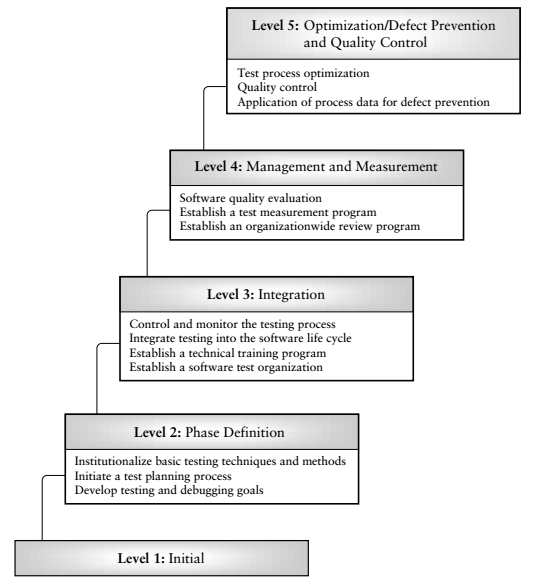
\includegraphics[scale=0.85]{img/TMMI}
    \caption{TMMi modelio brandos lygiai \cite{Burnstein:2010:PST:1965566}}
    \label{img:tmmi}
\end{figure}

\section{Programų sistemų kūrimo V-modeliu struktūra}
\begin{figure}[H]
    \centering
    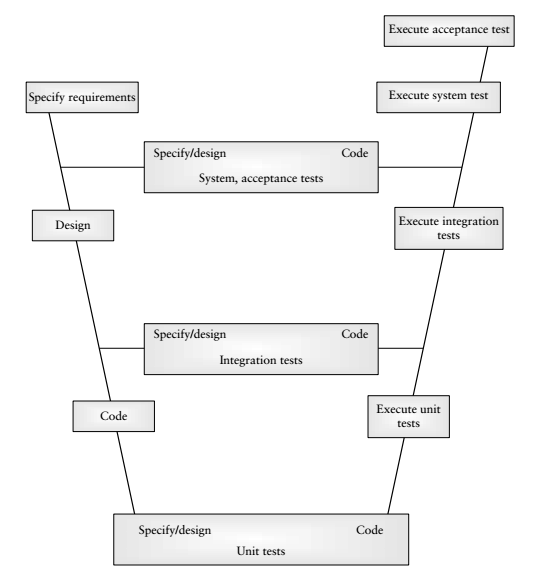
\includegraphics[scale=1]{img/Vmodel}
    \caption{V-modelis \cite{Burnstein:2010:PST:1965566}}
    \label{img:vmodel}
\end{figure}

\end{document}
